\documentclass[twocolumn,12pt]{article}

\usepackage[utf8]{inputenc}
\usepackage{graphicx}
\usepackage{amssymb}
\usepackage{amsmath}
\providecommand{\pr}[1]{\ensuremath{\Pr\left(#1\right)}}
\providecommand{\cbrak}[1]{\ensuremath{\left\{#1\right\}}}

\title{Assignment 5}
\author{Gollapudi Sasank CS21BTECH11019}

\begin{document}
\maketitle
\section*{Question : }
A die has two faces each with number \lq1\rq, three faces each with number \lq2\rq and one face with number \lq3\rq. If the die is rolled once, determine
\begin{enumerate}
\item P(2)
\item P(1 or 3)
\item P(not 3)
\end{enumerate}
\section*{Solution : }
Given the numbers present on the six faces of die are $ 1,1,2,2,2,3 $.\\
Let $S$ denote the Sample space of the experiment.\\
$\Rightarrow S = \{1,1,2,2,2,3\}$ \\
Let $X$ be the random variable that denotes the number obtained on the top when the die is rolled.\\
$\Rightarrow X \in \cbrak{1,2,3}$\\
\begin{align}
\pr{X=1} &= \frac{2}{6} = 0.33 \\
\pr{X=2} &= \frac{3}{6} = 0.5 \\
\pr{X=3} &= \frac{1}{6} = 0.166 
\end{align}
The Events $ X = 1 $ , $ X = 2 $ and $ X = 3 $ are mutually exclusive because when we roll a die exactly one of $ 1,2,3 $ appear at the top.
\begin{align}
\Rightarrow \pr{(X=i) \cap (X=j)} = 0\forall i,j \in \cbrak{1,2,3}
\end{align}
We know that for ant two events $ A,B$ \\
$ \pr{A \cup B} = \pr{A} + \pr{B} - \pr{A \cap B} $ \\
Let $ X=1 $ be the event $A$ and $X=3$ be the event $B$ \\
But here $\pr{A \cap B = 0} $ from (4)
\begin{align}
\Rightarrow \pr{A \cup B} &= \pr{A}+\pr{B} \\
\Rightarrow \pr{A \cup B}  &= \frac{2}{6} + \frac{1}{6} \\
\Rightarrow \pr{A \cup B} &= \frac{3}{6} \\
\Rightarrow \pr{A \cup B} &= 0.5 \\
\therefore \pr{(X=1) \cup (X=3)} = 0.5
\end{align}
We know that for any event $A$ it's complementary event is denoted by $A^{c}$\\
And $\pr{A} + \pr{A^{c}} = 1 $ \\
Let $X=3$ be the event $A$ \\
\begin{align}
\Rightarrow \pr{A^{c}}  = 1 - \pr{A} \\
\Rightarrow \pr{A^{c}}  = 1 - \frac{1}{6} \\
\Rightarrow \pr{A^{c}}  = \frac{5}{6} \\
\therefore \pr{(X=3)^{c}} = 0.88
\end{align}
\begin{figure}[h]
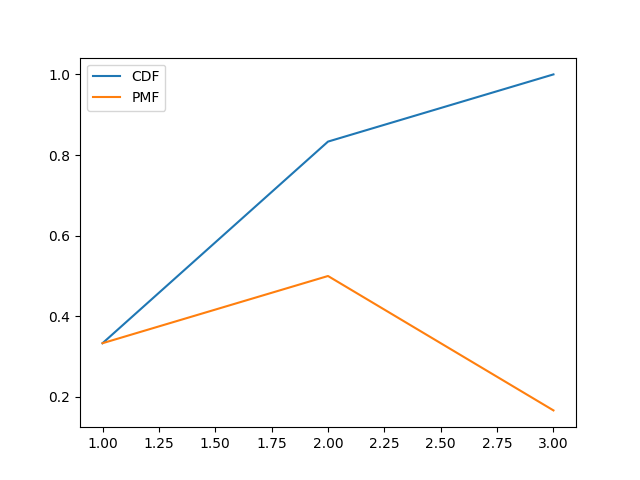
\includegraphics[width=\columnwidth]{fig1.png}
\caption{PMF and CDF the distribution}
\label{Fig 1}
\end{figure}
\end{document}
